\section{Исследование системы гидродинамики на основе метода функционала плотности \label{dhd}}
\subsection{Постановка задачи}
\subsubsection{Метод функционала плотности}
Рассмотрим задачу течения 2-х несмешиваемых жидкостей в керне. Движение жидкости описывается с помощью \textit{метода функционала плотности}. Система уравнений состоит из уравнений неразрывности и уравнения движения.
Подробное описание и теоретический вывод метода функционала плотности приведен в \cite{demyanov, dhd_spe}. Остановимся на результатах его применения, которые пригодятся в данной работе.
\par
Уравнения неразрывности каждой жидкости выражены через их мольные плотности - молярные массы на единицу объема. Если сложить их, можно получить стандартный вид уравнения неразрывности. 
Задача решается в кубе $D \in \mathbb{R}^3; t \in (0, T)$. Решение ищется в виде мольных плотностей $n_i = [n_1, n_2]^T$ и вектора среднемассовой скорости $v_a$. Все функции, из которых составлены уравнения, и неизвестные решения считаются гладкими.

\begin{equation} \label{eq:dhd_system}
\begin{cases}
\frac{\partial n_{i}}{\partial t}+\frac{\partial\left(V_{b}n_{i}\right)}{\partial x_{b}}-\frac{\partial}{\partial x_{b}}\left(P_{i j}\frac{\partial\Phi_{j}}{\partial x_{b}}\right)=\vartheta_{i}^{n}(t,x_{a}) 
\\ \\
\frac {\partial\rho V_{a}} {\partial t} + \frac {\partial} {\partial x_{b}} \left( \rho V_{b}V_{a} - \tau_{ab} \right) + n_i \frac{\partial \Phi_i}{\partial x_a}=\vartheta_{a}^{M}(t,x_{a})
\end{cases}
\end{equation}
где $\rho = M_i \cdot n_i$ - плотность ($M_i$ - молярные массы), $P_{ij}$ - матрица диффузии. $\vartheta^n_i$ и $\vartheta^M_a$ - источник плотности и внешняя сила. 
\\
$\tau_{ab}$ - тензор вязкости:
\begin{equation} \label{eq:viscosity_tensor}
\tau_{ab} = (\eta - \frac{2}{3} \mu) \frac {\partial V_c} {\partial x_c} \delta_{ab} + \mu \left( \frac{\partial V_{a}}{\partial x_{b}}+\frac{\partial V_{b}}{\partial x_{a}} \right) 
\end{equation}
где $\mu$ - сдвиговая вязкость, а $\eta$ - объемная вязкость.

\subsubsection*{Обобщенная свободная энергия}
В методе функционала плотности используется термодинамический потенциал - обобщенная свободная энергия:
\begin{equation} \label{eq:helmholz_energy}
w = f + \frac{1}{2} \nu_{ij} \frac {\partial n_i} {\partial x_a} \frac {\partial n_j} {\partial x_a}
\end{equation}
где $f = f(n_i)$ - свободная энергия смеси, а $\nu_{ij} = \nu_{ij} (n_i)$ - положительно определенная матрица, определяющая поверхностное натяжение между компонентами. Смесь стремится к наиболее выгодному состоянию, в котором обобщенная свободная энергия принимает минимальное значение. Исследуемые жидкости несмешиваемые. Поэтому $f(n_i)$ определятся так, чтобы иметь минимумы в точках, полностью заполненных одной жидкостью. Такие устойчивые состояния и есть \textit{фазы} в нашей модели. Мы рассматриваем двухфазную смесь - свободная энергия принимает минимальное значение, если в точке находится только одна из двух жидкостей.
\par
В рамках данной работы используется физическая модель двух жидкостей с такой свободной энергией:
\begin{equation}
\frac{1}{f} = \frac{1}{f_0} + \frac{1}{f_1}
\end{equation}
Где $f_i$ - свободная энергия каждой жидкости, задающаяся такой формулой:
\begin{equation}
f_i = (n_i - \overline n_i)^T E_i (n_i - \overline n_i)
\end{equation}
где $\overline n_i$ - мольные плотности в чистых фазах, $E_i$ - матрицы свободной энергии. Смысл данной формулы - сделать минимальной свободную энергию в фазе.
\par
Дифференцируя $w$  из формулы \eqref{eq:helmholz_energy} по $n_i$, получим обобщенный химический потенциал $\Phi$:
\begin{equation}
\Phi_i := \frac{\partial w}{\partial n_i} =\frac{\partial f}{\partial n_{i}}+\frac{1}{2}\frac{\partial\nu_{jk}}{\partial n_{i}}\frac{\partial n_{j}}{\partial x_{a}}\frac{\partial n_{k}}{\partial x_{a}}-\frac{\partial}{\partial x_{a}}\left(\nu_{ij}\frac{\partial n_{j}}{\partial x_{a}}\right)
\end{equation}
Через него можно выразить тензор напряжений:
\begin{equation}
\sigma_{ab} = (\omega-\Phi_{j}n_{j})\delta_{ab}-\nu_{ij}\frac{\partial n_{i}}{\partial x_{a}}\frac{\partial n_{j}}{\partial x_{b}}
\end{equation}
Отсюда получим давление:
\begin{equation}
p=-\frac{1}{3}\sum_a{\sigma_{aa}}=(\Phi_{j}n_{j}-\omega)+\sum_a{\frac{\nu_{ij}}{3}\frac{\partial n_{i}}{\partial x_{a}}\frac{\partial n_{j}}{\partial x_{a}}}
\end{equation}
\subsubsection{Сферическая симметрия}
В данной работе для проведения численных экспериментов рассматривается система функционала плотности в сферических координатах с учетом сферической симметрии. Такой подход позволяет решать численно одномерную систему и получать результаты, учитывающие влияние поверхностного натяжения. Получим вид системы \eqref{eq:dhd_system} в сферических координатах. В силу сферической симметрии все функции зависят только от $r$:
\begin{equation}
\frac{\partial}{\partial \theta} = 0;
\quad
\frac{\partial}{\partial \varphi} = 0 
\end{equation}
Воспользуемся выражениями для дивергенции, градиента и оператора Лапласа в сферических координатах c учетом симметрии:
\begin{equation}
\frac{\partial f_i}{x_i} \rightarrow \frac{1}{r^2} \frac{\partial}{\partial r} ( r^2 f_i );
\quad
\frac{\partial g}{x_i} \rightarrow \frac{\partial g}{\partial r};
\quad
\frac{\partial^2 \varphi}{\partial x_i \partial x_i} \rightarrow \frac{1}{r^2} \frac{\partial}{\partial r} \left( r^2 \frac{\partial \varphi}{\partial r} \right)
\end{equation}
Исследуемая система находится на отрезке $(0, R)$ на оси $r$, все векторы коллинеарны этой оси. Получим систему функционала плотности на этой оси:
\begin{equation} \label{eq:dhd_spherical}
\begin{cases}
\frac{\partial n_{i}}{\partial t} + \frac {1} {r^2} \frac{\partial}{\partial r}\left( r^2 \left[V_{r} n_{i} - P_{i j}\frac{\partial\Phi_{j}}{\partial r} \right] \right)=\vartheta_{i}^{n}(t, r) 
\\ \\
\frac {\partial\rho V_{r}} {\partial t} + \frac {1} {r^2} \frac {\partial} {\partial r} \left[ r^2 \left( \rho V_{r}^2 - \tau_{rr} \right) \right] + n_i \frac{\partial \Phi_i}{\partial r}=\vartheta^{M}(t, r)
\end{cases}
\end{equation}
В рамках данной работы мы принимаем в \eqref{eq:helmholz_energy} $\nu_{ij} = const$. Перепишем формулы для химического потенциала и вязкости:
\begin{equation}
\Phi_i = \frac{\partial f}{\partial n_i} - \nu_{ij} \left[ \frac{1}{r^2} \frac{\partial}{\partial r} \left( r^2 \frac{\partial n_j} {\partial r} \right) \right]
\end{equation}
\begin{equation}
\tau_{rr} = (\eta - \frac{2}{3} \mu) \frac{1}{r^2} \frac{\partial \left( r^2 V_r\right) }{\partial r} + 2\mu \frac{\partial V}{\partial r}
\end{equation}
где по индексу $r$ суммирование не ведется.
Таким образом, изучается трехмерная капля одной жидкости внутри другой с учетом сферической симметрии. При этом численно решается одномерная задача.

\subsubsection{Начальные и граничные условия \label{dhd:boundary_conditions}}
\paragraph{Начальные условия}
\begin{equation} \label{eq:initial_conditions_dhd}
n_i \vert_{t=0} = n_{i, 0} (x_i); \quad V_a \vert_{t=0} = V_{a, 0}(x_i)
\end{equation}

Рассматриваются 3 вида граничных условий: \textit{условия Дирихле}, \textit{условия камня} и \textit{условия симметрии}:
\paragraph{Условия Дирихле}
\begin{equation} \label{eq:dirichlet_dhd}
n_i \vert_{\partial D} = n_{i, 0}(r); \quad \left. V_r \right \vert_{\partial D} = V_{r, 0}(r) 
\end{equation}
\paragraph{Условия камня} используются для моделирования твердой стены, через которую не может течь жидкость. В рамках сферической симметрии его можно использовать на внешней границе. Для реализации условия камня необходимо приравнять к нулю скорости на границе клеток камня, мольные концентрации внутри камня: 
\begin{equation}
n_i \vert_{\textrm{rock}} = 0;
\quad \quad
V_r \vert_{\textrm{rock}} = 0
\end{equation}
Потока через каменную границу быть не должно. Рассмотрим, из каких слагаемых состоит поток в уравнении \eqref{eq:dhd_spherical}. Все компоненты, кроме одной, приравняются к нулю сами. Диффузионный поток на границе с камнем нужно приравнять к нулю вручную:
\begin{equation}
\left. P_{ij} \cdot \frac{\partial \Phi_j}{\partial r} \right \vert_{\textrm{rock}} = 0
\end{equation}
\paragraph{Условия симметрии} используются в центре сферической симметрии. Скалярные поля должны быть симметричны относительно центра капли, а векторные --- антисимметричны. Центр находится в точке $r = 0$:
\begin{equation} \label{eq:symmetry}
\left. \left. \frac{\partial n_i (r, t)} {\partial r} \right \vert_{r=0} = 0; 
\quad \quad
V_r(r, t) \right \vert_{r=0} = 0
\end{equation}
\subsection{Дискретизация \label{dhd:discretization}}
Второй порядок аппроксимации достигается методом, описанным в главе \ref{methods:space_derivative}. Используем постоянный шаг $h$ для сеток по пространству. Введем названия для разных сеток:
\begin{itemize}
\item D-точки находятся в центрах ячеек: $\quad r^D_{i} = \left[ \frac{h}{2} + h \cdot i\right] \quad \quad i = \overline{0, M-1}$
\item U-точки находятся на гранях между ячейками: $\quad r^U_{i} = \left[ h \cdot i\right] \quad \quad i = \overline{0, M}$
\end{itemize}
Значения $n_i$ определяются в D-точках, $V_r$ --- в U-точках.
\par
Введем операторы интерполяции $I^D$, $I^U$ с одной сетки на другую. Верхний индекс указывает, с какой сетки происходит интерполяция. Аналогичным образом введем операторы производной с разных сеток: $D^{\times} \approx \frac {\partial } {\partial r}$. Здесь $\times$ - либо D, либо U. Данный оператор переносит значения на другую сетку, так как использует формулу центральной разности --- значение производной вычисляется посередине между соседними точками для повышения точности. Приведем примеры действия операторов на вектор $q^\times$ на рис. \ref{fig:dhd_points}
\begin{figure}[H]
  \centering
  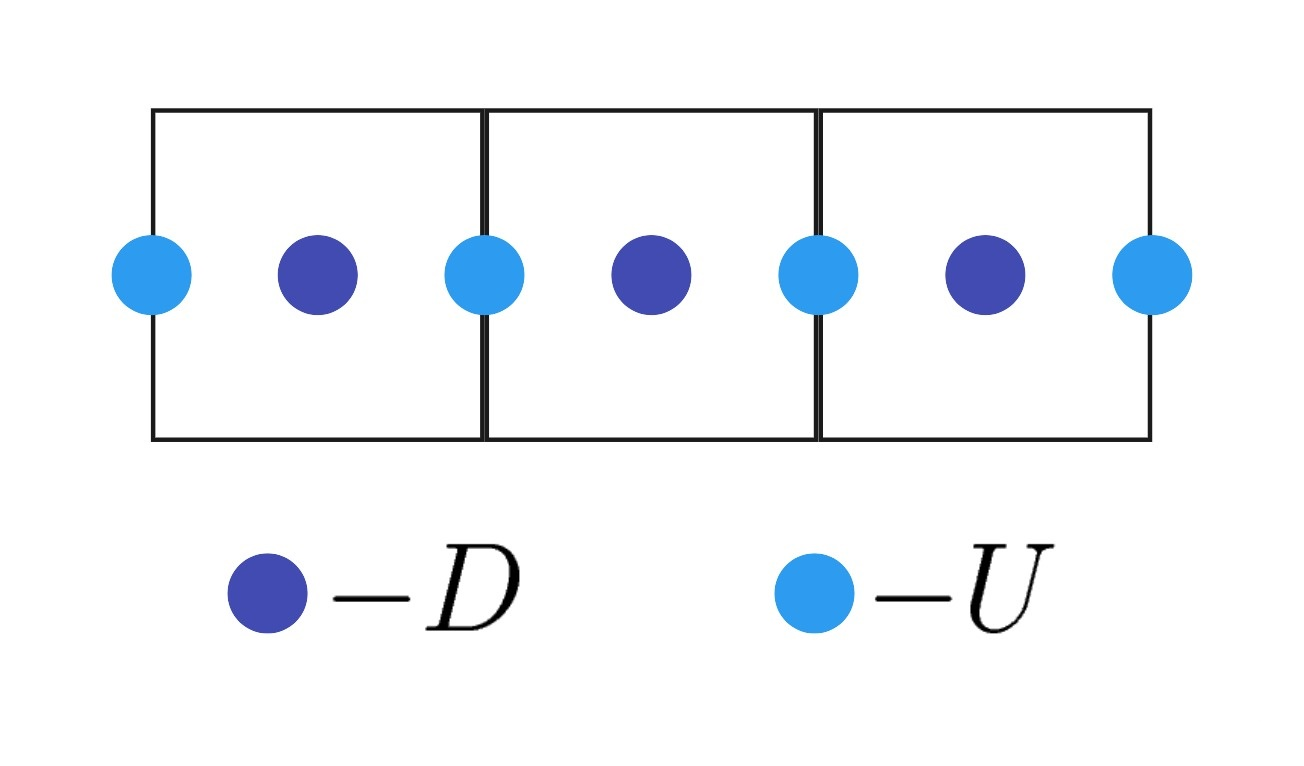
\includegraphics[valign = c, width = .5\linewidth]{common_images/dhd_points.jpg} \qquad
  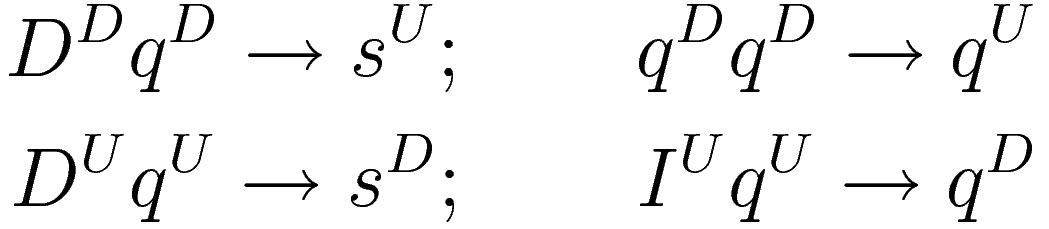
\includegraphics[width = .3\linewidth]{common_images/dhd_interpolation.png}
  \caption{Визуализация точек на разных сетках и примеры действия операторов интерполяции и дифференцирования}
  \label{fig:dhd_points}
\end{figure}

\subsubsection*{Аппроксимация граничных условий симметрии} 
Центр симметрии на левой границе (рис. \ref{fig:dhd_symmetry}). Граница расположена между соседними D-точками, чтобы аппроксимировать производную от $n_i$ по формуле центральной разности. Однако для расчета нужна крайняя U-точка, которая находится левее последней D-точки. Поэтому необходимо использовать дополнительную U-точку в $r = -h$. Значение вектора $V_r$ в ней определяется из соображений симметрии --- он должен быть направлен противоположено $V_r(h)$. Получаем дискретный вид граничных условий симметрии:
\begin{equation}
n_{i, 0} = n_{i, 1};
\quad \quad
V_{r, 0} = -V_{r, 2};
\quad \quad
V_{r, 1} = 0
\end{equation}
\begin{figure}[H]
\centering
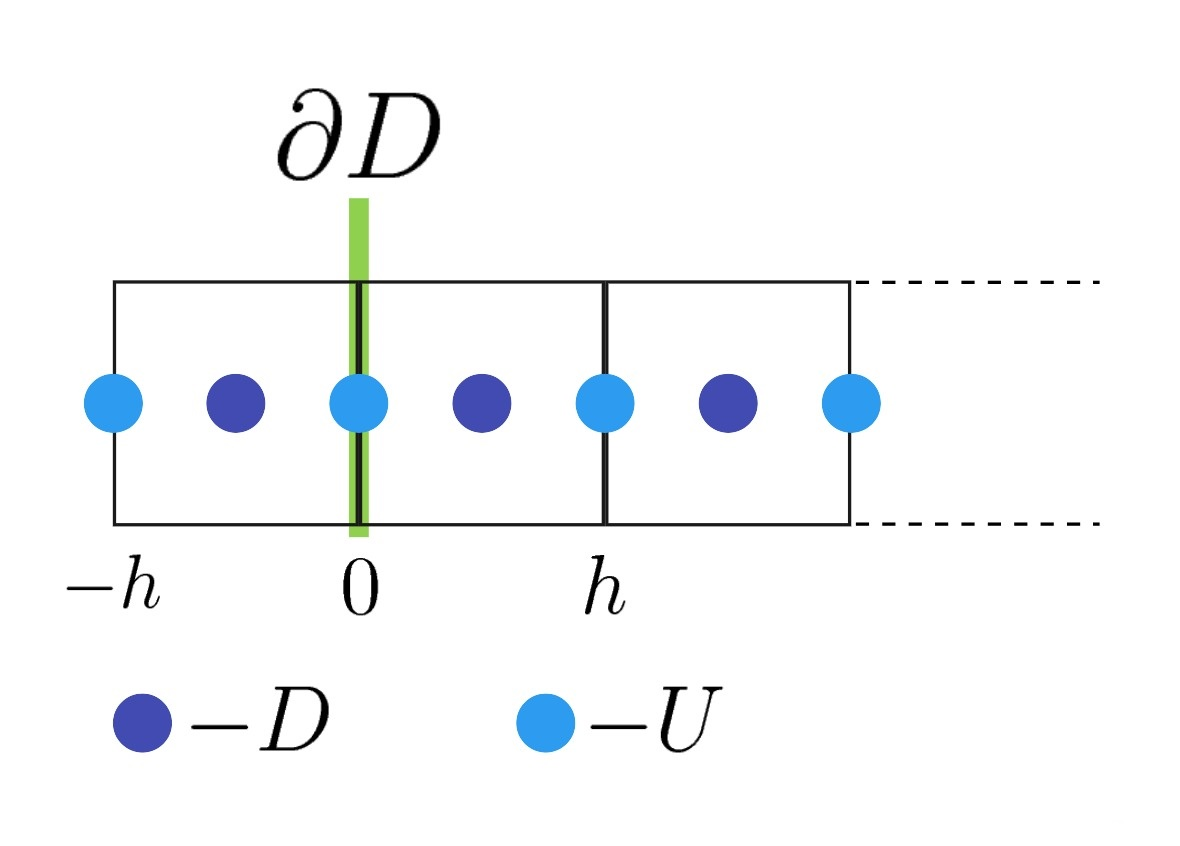
\includegraphics[width=0.5\textwidth]{common_images/symmetry.jpg}
\caption{Граничное условие симметрии. Внизу подписан тип точек.}
\label{fig:dhd_symmetry}
\end{figure}

\subsection{Особенности реализации численных схем \label{dhd:features}}
Запишем численно задачу функционала плотности \eqref{eq:dhd_system} в терминах производных на разных сетках из раздела \ref{dhd:discretization}. 
\begin{equation} \label{eq:dhd_difference}
\begin{cases}
\frac{\partial n_i}{\partial t} + \frac {1} {r^2} D^U_0 \left[ r^2 \left( V_r \cdot I^D_0 n_i - P_{ij} \cdot D^D_0 \Phi_j\right) \right] = \vartheta_{i}^{n}
\\ \\
\frac{\partial \left( \rho(I^D_0 n_i) \cdot V_r \right)}{\partial t} + \frac{1}{r^2} D^U_0 \left[ r^2 \left( \rho(n_i) \cdot I^U_0 V^2_r - \tau_{rr} \right) \right] + I^D_0 n_i \cdot D^D_0 \Phi_i = \vartheta^M
\end{cases}
\end{equation}
Для удобства функции от $n_i$ и $V_r$ определены на тех сетках, на которых они нужны в системе \eqref{eq:dhd_difference}. Покажем, как они вычисляются численно. Будем использовать верхний индекс, для уточнения сетки, например $n^D_i$ и $V_r^U$:
\begin{equation}
P_{ij}^U = P_{ij} \left( I^D_0(n_i) \right)
\end{equation}
\begin{equation}
\tau_{rr}^D = (\eta - \frac{2}{3} \mu) \frac{1}{r^2} D^U_0 \left( r^2 V_r \right) + 2 \mu D^U_0 V_r
\end{equation}
\begin{equation}
\Phi^D_i = \frac{\partial f}{\partial n} - \nu_{ij} \frac{1}{r^2} \left( r^2 \frac{\partial n_j}{\partial r} \right)
\end{equation}
Функция $\rho$ указана в системе \eqref{eq:dhd_difference} со своими аргументами в явном виде, поскольку используется на разных сетках.
\subsubsection*{Интегрирование по времени}
Аппроксимация производной по времени методами из раздела \ref{methods:time_integration} приводит либо к явному, либо к неявному методу решения. В рамках данной работы реализованы оба этих метода. Анализ устойчивости уравнения \eqref{eq:dhd_system} показывает, что шаг по времени $\tau$ существенно ограничен для явного метода. Поэтому интерес для исследования представляет решение неявным методом. 
\subsubsection*{Неявное решение}
Рассмотрим используемый алгоритм неявного решения согласно главе \ref{methods}:
\begin{itemize}
\renewcommand{\labelitemii}{•}
% \renewcommand{\labelitemiii}{•}
    \item Цикл шагов по времени 
    \begin{itemize}
        \item Цикл итераций метода Ньютона (раздел \ref{methods:newton})
        \begin{itemize}
            \item Цикл итераций метода решения линейной системы (раздел \ref{methods:linear_solvers})
            \item Перерасчет матрицы Якоби, если необходимо (раздел \ref{implementation:operator_preconditioning})
        \end{itemize}
    \end{itemize}
\end{itemize}
Матрица Якоби не обладает тридиагональным видом \eqref{mat:tridiagonal}, несмотря на то, что система одномерная. Причина в том, что вектор неизвестных в системе \eqref{eq:newtons_method_system} включает в себя как $n_i$, так и $V_r$: 
\begin{equation}
\mathbf{x} = \left[ n_0 \dots n_{0, M-1}; \quad n_1 \dots n_{1, M-1}; \quad V_{r, 0} \dots V_{r, M}\right]
\end{equation}
Здесь  $M$ - количество D-точек, $M+1$ - количество U-точек. Нелинейная система $\mathbf{F}(\mathbf{x}) = 0$ связывает $n_0$, $n_1$ и $V_r$ зависимостью. Кроме того, в системе присутствует 4-я производная. Она приводит к зависимости значений в 5 точках друг от друга. Поэтому необходимо применять общие методы решения разреженных линейных систем, рассмотренные ранее. Будем использовать  \textit{методы подпространства Крылова}. Матрица Якоби не симметрична, поэтому нам подойдут методы GMRES или BiCGStab (разделы \ref{methods:gmres}, \ref{methods:bicgstab}).
\subsubsection*{Вычисление действия матрицы Якоби}
Поскольку мы используем {методы подпространства Крылова}, мы можем вычислить матрицу Якоби в виде оператора, способного действовать на вектор. Реализованы численный и аналитический подходы, описанные в главе \ref{implementation:operator_preconditioning}.
Прямой метод используется для проверки аналитического.
Рассмотрим, как дифференцируется сложная функция $\mathbf{F}(\mathbf{x})$ для системы функционала плотности, записанной численно \eqref{eq:dhd_difference}:
\begin{equation} 
    \left\{
        \begin{multlined}
            d\frac{\partial n_i}{\partial t} + \frac {1} {r^2} D^U_0 \left[ r^2 \left( dV_r \cdot I^D_0 n_i + V_r \cdot I^D_0 dn_i - dP_{ij} \cdot D^D_0 \Phi_j - P_{ij} \cdot D^D_0 d\Phi_j\right) \right] = 0 
            \\ \\
            \shoveleft{
                d\frac{\partial \left( \rho(I^D_0 n_i) \cdot V_r \right)}{\partial t} + \frac{1}{r^2} D^U_0 \left[ r^2 \left( d\rho(n_i) \cdot I^U_0 V^2_r + \rho(n_i) \cdot I^U_0 (2V_r dV_r) - d\tau_{rr} \right) \right] +
            }
            \\
            +  I^D_0 dn_i \cdot D^D_0 \Phi_i + I^D_0 n_i \cdot D^D_0 d\Phi_i = 0
        \end{multlined}
    \right.
\end{equation}
Здесь дифференциал от $\frac{\partial}{\partial t}$ мы оставили в общем виде, поскольку его вид зависит от выбранной дискретизации. Важно, что только значения на нелинейном слое по времени считаются функциями, по которым происходит дифференцирование. Значения на известных предыдущих слоях входят в решаемую систему $\mathbf{F}(\mathbf{x}) = 0$ уже как константы. Например, для неявного метода Эйлера (раздел \ref{methods:time_integration}):
\begin{equation}
     d\frac{\partial n_i}{\partial t} = \frac{dn_i}{\tau}; 
     \quad
     d\frac{\partial \left( \rho(I^D_0 n_i) \cdot V_r \right)}{\partial t} = \frac{d\rho(I^D_0 n_i) \cdot V_r + \rho(I^D_0 n_i) \cdot dV_r}{\tau}
\end{equation}
Дифференциалы функций $\rho, P_{ij}, \Phi_i, \tau_{rr}$ рассчитываются аналогично. Покажем на примере $\rho$:
\begin{equation}
d \rho = d\left( M_i n_i \right) = M_i dn_i
\end{equation}

\subsubsection*{Особенности применения предобуславливателей}
При расчетах мы пользовались такими предобуславливателями: полный метод LU, разреженный метод ILU и многосеточный метод (разделы \ref{methods:lu}, \ref{methods:ilu}, \ref{methods:multigrid}). Полный метод не занимает слишком много времени, так как система одномерная. По сравнению с ним, разреженный метод не дает прироста производительности в одномерной задаче. Однако такой подход плохо масштабируется, поэтому мы рассмотрели многосеточный метод.
\par
Применение многосеточного метода отличается от его применения к скалярной задаче теплопроводности \eqref{eq:heat_equation}. При построении векторного оператора интерполяции на более грубую сетку необходимо учесть, что в одном векторе переменных нелинейной системы $\mathbf{x}$ содержатся значения $n_0$, $n_1$ и $V_r$. Именно этим методом планируется решать трехмерную систему функционала плотности \eqref{eq:dhd_system}, поскольку там размер матрицы будет значительно больше.

\subsubsection*{Компиляция кода}
В формуле \eqref{eq:dhd_difference} используются аналитические гладкие функции, например производная свободной энергии $\frac{\partial f}{\partial n_i}$. Согласно подходу, описанному в разделе \ref{implementation:cuda}, такие производные вычисляются аналитически с помощью символьной математики. Для использования физической модели жидкости достаточно задать вид свободной энергии. Результатом описанного подхода является сгенерированная формула на языке С с атрибутами CUDA, которая встраивается в численную схему. Покажем, как выглядит код таких формул на примере производной свободной энергии $\frac{\partial f}{\partial n_i}$ для конкретной жидкости:
\begin{lstlisting}[style=CStyle]
static __device__
void compute_chemical_potentials(double *n, double *dw) {
   dw[0] = 2.1780926979276557e-6*(-69.757105602213599*n[0] - 418.78244767971137*n[1] + 3594.1684922005115)*((n[0] - 55.555555555555557)*(16.199999999999999*n[0] - 900.
   0) + 97.255693077323699*(n[0] - 55.555555555555557)*n[1] + (97.255693077323699*n[0] - 5403.0940598513171)*n[1] + 677.58193767828004*pow(n[1], 2))*((n[1] - 8.0)*
   (781.25*n[1] - 6250.0) + 112.135530762532*(n[1] - 8.0)*n[0] + (112.135530762532*n[1] - 897.084246100256)*n[0] + 18.6785528011068*pow(n[0], 2))/pow(0.
   0014758362707047335*(n[0] - 55.555555555555557)*(16.199999999999999*n[0] - 900.0) + 0.14353347937604158*(n[0] - 55.555555555555557)*n[1] + 0.0014758362707047335*
   (97.255693077323699*n[0] - 5403.0940598513171)*n[1] + 0.0014758362707047335*(n[1] - 8.0)*(781.25*n[1] - 6250.0) + 0.16549368353407115*(n[1] - 8.0)*n[0] + 0.
   0014758362707047335*(112.135530762532*n[1] - 897.084246100256)*n[0] + 0.027566485708146914*pow(n[0], 2) + pow(n[1], 2), 2) + (32.399999999999999*n[0] + 194.
   5113861546474*n[1] - 1800.0)*((n[1] - 8.0)*(781.25*n[1] - 6250.0) + 112.135530762532*(n[1] - 8.0)*n[0] + (112.135530762532*n[1] - 897.084246100256)*n[0] + 18.
   6785528011068*pow(n[0], 2))/((n[0] - 55.555555555555557)*(16.199999999999999*n[0] - 900.0) + 97.255693077323699*(n[0] - 55.555555555555557)*n[1] + (97.
   255693077323699*n[0] - 5403.0940598513171)*n[1] + (n[1] - 8.0)*(781.25*n[1] - 6250.0) + 112.135530762532*(n[1] - 8.0)*n[0] + (112.135530762532*n[1] - 897.
   084246100256)*n[0] + 18.6785528011068*pow(n[0], 2) + 677.58193767828004*pow(n[1], 2)) + (37.357105602213601*n[0] + 224.271061525064*n[1] - 1794.168492200512)*((n
   [0] - 55.555555555555557)*(16.199999999999999*n[0] - 900.0) + 97.255693077323699*(n[0] - 55.555555555555557)*n[1] + (97.255693077323699*n[0] - 5403.0940598513171)*n
   [1] + 677.58193767828004*pow(n[1], 2))/((n[0] - 55.555555555555557)*(16.199999999999999*n[0] - 900.0) + 97.255693077323699*(n[0] - 55.555555555555557)*n[1] + (97.
   255693077323699*n[0] - 5403.0940598513171)*n[1] + (n[1] - 8.0)*(781.25*n[1] - 6250.0) + 112.135530762532*(n[1] - 8.0)*n[0] + (112.135530762532*n[1] - 897.
   084246100256)*n[0] + 18.6785528011068*pow(n[0], 2) + 677.58193767828004*pow(n[1], 2)) + ((n[1] < 0) ? (
      20.0*n[0]*pow(n[1], 2)
   )  : (0)) + ((n[0] < 0) ? (
      20.0*(pow(n[0], 2) + pow(n[1], 2))*n[0] + 20.0*pow(n[0], 3)
   ) : (0));
   dw[1] = 2.1780926979276557e-6*(-418.78244767971142*n[0] - 2917.6638753565603*n[1] + 23306.188119702638)*((n[0] - 55.555555555555557)*(16.199999999999999*n[0] - 900.
   0) + 97.255693077323699*(n[0] - 55.555555555555557)*n[1] + (97.255693077323699*n[0] - 5403.0940598513171)*n[1] + 677.58193767828004*pow(n[1], 2))*((n[1] - 8.0)*
   (781.25*n[1] - 6250.0) + 112.135530762532*(n[1] - 8.0)*n[0] + (112.135530762532*n[1] - 897.084246100256)*n[0] + 18.6785528011068*pow(n[0], 2))/pow(0.
   0014758362707047335*(n[0] - 55.555555555555557)*(16.199999999999999*n[0] - 900.0) + 0.14353347937604158*(n[0] - 55.555555555555557)*n[1] + 0.0014758362707047335*
   (97.255693077323699*n[0] - 5403.0940598513171)*n[1] + 0.0014758362707047335*(n[1] - 8.0)*(781.25*n[1] - 6250.0) + 0.16549368353407115*(n[1] - 8.0)*n[0] + 0.
   0014758362707047335*(112.135530762532*n[1] - 897.084246100256)*n[0] + 0.027566485708146914*pow(n[0], 2) + pow(n[1], 2), 2) + (194.5113861546474*n[0] + 1355.
   1638753565601*n[1] - 10806.188119702634)*((n[1] - 8.0)*(781.25*n[1] - 6250.0) + 112.135530762532*(n[1] - 8.0)*n[0] + (112.135530762532*n[1] - 897.084246100256)*n
   [0] + 18.6785528011068*pow(n[0], 2))/((n[0] - 55.555555555555557)*(16.199999999999999*n[0] - 900.0) + 97.255693077323699*(n[0] - 55.555555555555557)*n[1] + (97.
   255693077323699*n[0] - 5403.0940598513171)*n[1] + (n[1] - 8.0)*(781.25*n[1] - 6250.0) + 112.135530762532*(n[1] - 8.0)*n[0] + (112.135530762532*n[1] - 897.
   084246100256)*n[0] + 18.6785528011068*pow(n[0], 2) + 677.58193767828004*pow(n[1], 2)) + (224.271061525064*n[0] + 1562.5*n[1] - 12500.0)*((n[0] - 55.555555555555557)
   *(16.199999999999999*n[0] - 900.0) + 97.255693077323699*(n[0] - 55.555555555555557)*n[1] + (97.255693077323699*n[0] - 5403.0940598513171)*n[1] + 677.
   58193767828004*pow(n[1], 2))/((n[0] - 55.555555555555557)*(16.199999999999999*n[0] - 900.0) + 97.255693077323699*(n[0] - 55.555555555555557)*n[1] + (97.
   255693077323699*n[0] - 5403.0940598513171)*n[1] + (n[1] - 8.0)*(781.25*n[1] - 6250.0) + 112.135530762532*(n[1] - 8.0)*n[0] + (112.135530762532*n[1] - 897.
   084246100256)*n[0] + 18.6785528011068*pow(n[0], 2) + 677.58193767828004*pow(n[1], 2)) + ((n[0] < 0) ? (
      20.0*pow(n[0], 2)*n[1]
   ) : (0 )) + ((n[1] < 0) ? (20.0*(pow(n[0], 2) + pow(n[1], 2))*n[1] + 20.0*pow(n[1], 3)) : (0));
}
\end{lstlisting}
Данный пример наглядно показывает необходимость использования символьной математики. Без нее для внедрения новых физических моделей жидкостей приходилось бы каждый раз вручную вычислять огромное количество производных и писать их на низкоуровневом языке. 
\par
Может показаться необычной подстановка численных значений для конкретной модели в исходный код. Следует объяснить, что данный код генерируется для каждой новой жидкости заново автоматически, а использование численных значений в исходном коде в перспективе дает компилятору простор для оптимизаций.
\subsection{Численные эксперименты}
Для всех численных экспериментов используются одни и те же настройки жидкостей:
\begin{itemize}
\item Молярные массы: $M_0 = 18, M_1 = 100$
\item Мольные плотности: $n_0 = 55.6, n_1 = 8$
\item Матрицы свободных энергий: \begin{equation}
E_0 = \left[
\begin{array}{cc}
16.2 & 97.2556930773237 \\
		97.2556930773237 & 677.58193767828
\end{array}
\right]
\end{equation}\begin{equation}
E_1 = \left[
\begin{array}{cc}
	18.6785528011068 & 112.135530762532 \\
	112.135530762532 & 781.25
\end{array}
\right]
\end{equation}
\item Матрица поверхностного натяжения: \begin{equation} \nu_{ij} =\left[
\begin{array}{cc}
\expnumber{1.87382211559043}{-10} & 0 \\
		0 & \expnumber{1.87382211559043}{-10}
\end{array}
\right] \end{equation}
\item Сдвиговые вязкости: $\mu_i  = \left[ 0.002, 0.001 \right]$
\item Объемные вязкости: $\eta_i = \left[ 0.021, 0.042 \right]$
\end{itemize}
Вязкости смеси, используемые в формуле тензора вязкости \eqref{eq:viscosity_tensor}, вычисляются по формулам:
\begin{multline}
\mu = \left(\frac{\mu_0^{1/3} \left(\left(n_0\right)^{2} + \left(n_1 - \overline n_1\right)^{2}\right)^{0.5}}{\left(\left(n_0 - \overline n_0\right)^{2} + \left(n_1\right)^{2}\right)^{0.5} + \left(\left(n_0\right)^{2} + \left(n_1 - \overline n_1\right)^{2}\right)^{0.5}} + \right.
\\
\left. + \frac{\mu_1^{1/3} \left(\left(n_0 - \overline n_0\right)^{2} + \left(n_1\right)^{2}\right)^{0.5}}{\left(\left(n_0 - \overline n_0\right)^{2} + \left(n_1\right)^{2}\right)^{0.5} + \left(\left(n_0\right)^{2} + \left(n_1 - \overline n_1\right)^{2}\right)^{0.5}}\right)^{3}
\end{multline}

\begin{multline}
\nu = \left(\frac{\nu_0^{1/3} \left(\left(n_0\right)^{2} + \left(n_1 - \overline n_1\right)^{2}\right)^{0.5}}{\left(\left(n_0 - \overline n_0\right)^{2} + \left(n_1\right)^{2}\right)^{0.5} + \left(\left(n_0\right)^{2} + \left(n_1 - \overline n_1\right)^{2}\right)^{0.5}} + \right.
\\
\left. + \frac{\nu_1^{1/3} \left(\left(n_0 - \overline n_0\right)^{2} + \left(n_1\right)^{2}\right)^{0.5}}{\left(\left(n_0 - \overline n_0\right)^{2} + \left(n_1\right)^{2}\right)^{0.5} + \left(\left(n_0\right)^{2} + \left(n_1 - \overline n_1\right)^{2}\right)^{0.5}}\right)^{3}
\end{multline}
\par
Матрица диффузии составляется таким образом, чтобы при диффузии не происходило переноса массы. За перенос массы отвечает среднемассовая скорость $V_r$. В данной работе используется формула:

\begin{equation}
    D_{ij} = \frac{5.0 \cdot 10^{-7}}{M^2_0} \cdot \left[\begin{matrix} M_1^{2} & - M_1 M_0\\- M_1 M_0 & M_0^2 \end{matrix}\right]
\end{equation}
В экспериментах использовались такие численные алгоритмы:
\begin{itemize}
\item Интегрирование по времени неявным методом 2 порядка по 3 точкам (раздел \ref{methods:back-diff})
\item Метод Ньютона решения нелинейной системы (раздел \ref{methods:newton})
\item Алгоритм GMRES решения СЛАУ (раздел \ref{methods:gmres})
\item Предобуславливатель LU (раздел \ref{methods:lu})
\item Действие матрицы Якобы вычислялось аналитическим методом, значения матрицы не хранились (раздел \ref{methods:computing_jacobi})
\end{itemize}

\paragraph{Выбор шага по времени и пространству} Во всех экспериментах, кроме исследования сеточной сходимости, шаг по времени $\tau$ выбирался таким образом. Задавался начальный шаг по времени $\tau_0$. С каждым шагом $\tau$ увеличивался на 10\%. Так $\tau$ доходил до такого значения, когда метод Ньютона не сходился. Тогда $\tau$ уменьшался на 10\%, пока методу Ньютона не удавалось сойтись. Стандартный шаг по пространству $h = \expnumber{2.4}{-6}$.

\subsubsection{Автоматическое тестирование}
Перечислим методы автоматического тестирования из раздела \ref{implementation:testing}, которые реализованы в данной задаче:
\begin{itemize}
\item Тестируются операторы производной
\item Решение неявным методом сравнивается с явным решением
\item Проверяется закон сохранения массы в задачах без источников
\end{itemize}
Закон сохранения массы проверялся с учетом сферических координат по формуле:
\begin{equation}
m = \int_{D} \rho(\mathbf{x}) d\mathbf{x} = \int_0^\pi \sin(\theta) d\theta \int_0^{2\pi} d\varphi \int_0^R r^2 \rho(r) dr \approx 4\pi h \sum_{i=0}^{M-1} r_i^2 \rho_i
\end{equation}

\subsubsection{Распад \label{dhd:interface}}
Исследуемые жидкости несмешиваемые. Поэтому при любых начальных условиях, если в задаче нет источников, мы ожидаем увидеть одно и то же стационарное решение --- смесь из двух жидкостей распадется на отдельные фазы. 
\par
Возьмем граничные условия (раздел \ref{dhd:boundary_conditions}): \textit{симметрия} слева и \textit{камень} справа. Заполним расчетную область равномерной смесью двух жидкостей. Разобьем расчетную область на 100 точек.
Сначала жидкость разваливается на капли, а затем образуется стабильная граница между двумя жидкостями. Рассмотрим, как эволюционирует такая система на рис. \ref{fig:decay}.
\begin{figure}[H]
\centering
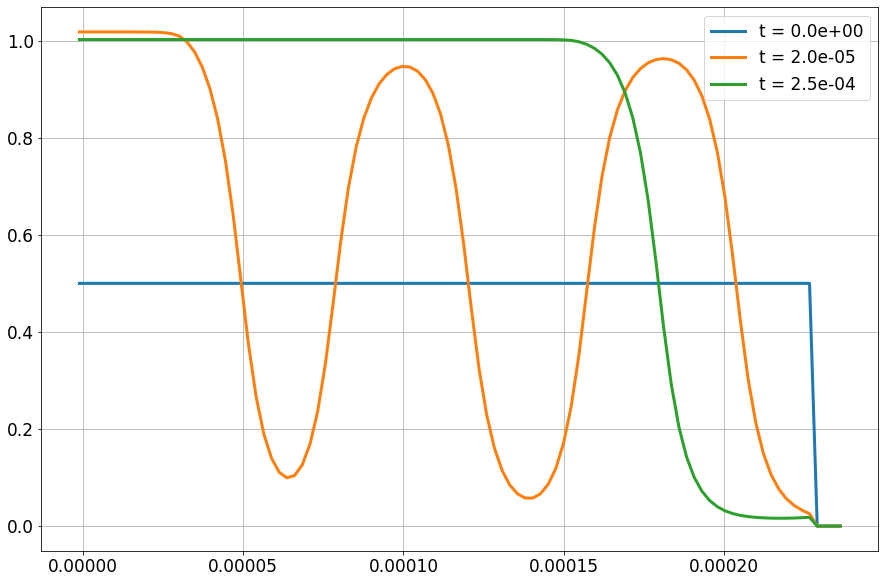
\includegraphics[width=.7\textwidth]{dhd_decay/decay.png}
\caption{Установление интерфейса между жидкостями. Показано процентное содержание первой жидкости в разные моменты времени.}
\label{fig:decay}
\end{figure}
\subsubsection{Кросс-валидация}
Реализованная программа численного решения системы функционала плотности \eqref{eq:dhd_spherical} сравнивается с результатами симулятора \textit{DHD 3D}, описанного в публикации \cite{dhd_spe}. Данная программа реализует физическую модель, описываемую системой функционала плотности \eqref{eq:dhd_system}. Перечислим особенности численной схемы \textit{DHD 3D}:
\begin{itemize}
\item Явный метод
\item Декартова система координат
\item 3D область пространства
\item Шаг по пространству $h = \expnumber{2.4}{-6}$
\item Шаг по времени $\tau = \expnumber{1}{-10}$
\end{itemize}
\paragraph{Постановка эксперимента}
Стационарное распределение мольных плотностей берется из эксперимента \ref{dhd:interface}. Делается линейная интерполяция в 3D сферу. Далее производится расчет \textit{DHD 3D}, используя эту сферу как начальное условие. Так как программы реализуют одну и ту же физическую модель, интерфейс не должен измениться.
\par
На рис. \ref{fig:cross_validation_vals} отложены значения относительной мольной плотности первой жидкости по оси, исходящей из центра капли. Значения нормированы на мольную плотность в чистой фазе. На графике показывается процентное содержание первой жидкости в зависимости от $r$. Черным цветом обозначено стационарное распределение, полученное в данной работе неявным методом. Другими цветами обозначены немного изменившиеся распределения после 3D расчета. Синим цветом обозначены значения, взятые по оси $x$, а желтым - лежащие под углом $45^\circ$ к оси $x$ в плоскости $xy$. 
\begin{figure}[h]
\centering
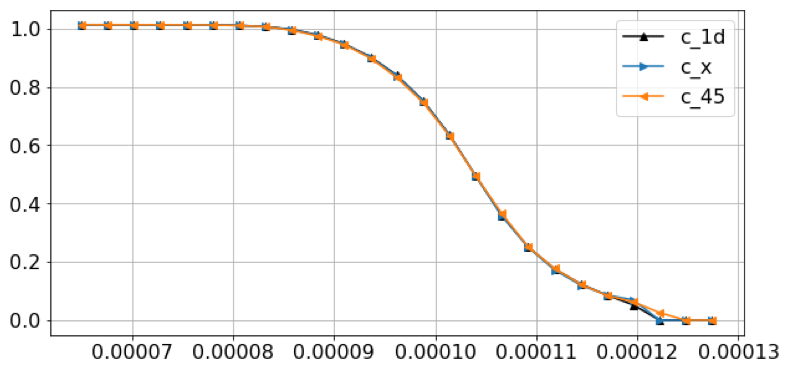
\includegraphics[scale=0.8]{dhd_cross_validation/cross_validation_vals.png}
\caption{Результаты расчета в 3d по разным осям и одномерный интерфейс}
\label{fig:cross_validation_vals}
\end{figure}
\par
Разница между этими значениями и исходным одномерным распределением показана на рис. \ref{fig:cross_validation_error}.
\begin{figure}[h]
\centering
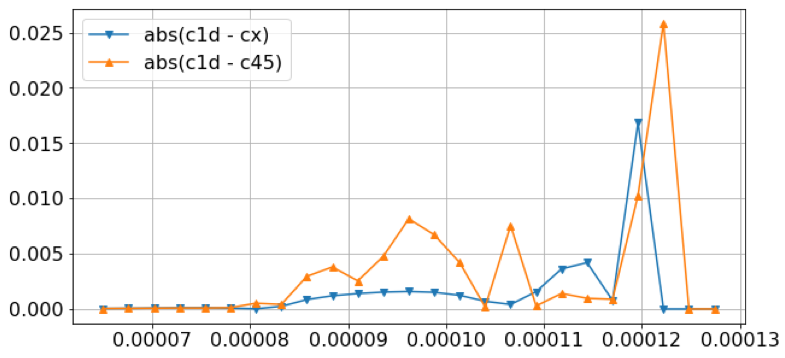
\includegraphics[scale=0.8]{dhd_cross_validation/cross_validation_error.png}
\caption{Ошибки по разным осям}
\label{fig:cross_validation_error}
\end{figure}
Основная ошибка образуется у границы. Это связано с дискретизацией границ сферы на регулярной сетке. На графике видно, что ошибка по оси $45^\circ$ больше, чем по оси $x$. Из этого делаем вывод, что основная ошибка связана с интерполяцией сферических координат в 3D.

\subsubsection{Исследование сеточной сходимости \label{dhd:convergence}}
\paragraph{Постановка эксперимента}
Проведем исследование сходимости неявной симуляции, воссоздав задачу из известного решения. Построим аналитическое решение из таких соображений. Есть некоторое распределение масс, которое перемещается из центра со скоростью $V_r(r)$:
\begin{equation}
V_r(r) = \frac{R} {10 T}  \left(1 + \operatorname{erf} \left[\frac{20} {R} \left( r - \frac{1}{2} R \right)  \right] \right)
\end{equation}
Для построения распределения масс используется функция $S(r, t)$:
\begin{equation}
S(r, t) = \left(\frac{1}{2} + \frac{1}{2} \operatorname{erf} \left[ \frac{20}{R} \left( r - t \cdot V_r(r) - {\frac{1}{2}R} \right) \right] \right)
\end{equation}
Из которой строятся поля мольных плотностей:
\begin{equation}
\begin{cases}
n_0 = \overline{n_0} \cdot S(r, t) 
\\
n_1 = \overline{n_1} \cdot (1 - S(r, t))
\end{cases}
\end{equation}
где $R = r_{max}$ и $T = t_{max}$, $\operatorname{erf}$ - интеграл распределения Гаусса (функция ошибок), $\overline{n_i}$ - мольные плотности в чистых фазах. Численные коэффициенты в формулах выбраны так, чтобы функции имели вид, показанный на рис. \ref{fig:dhd_convergence_analytic}. 
\begin{figure}[H]
\centering
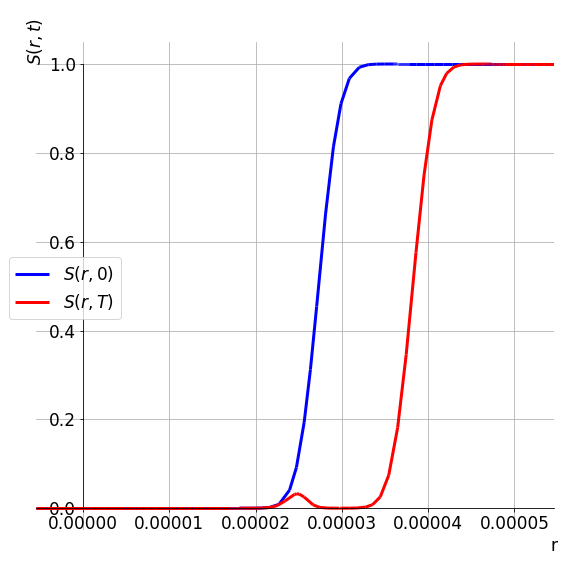
\includegraphics[width=.4\textwidth]{dhd_convergence/analytic_n.png}
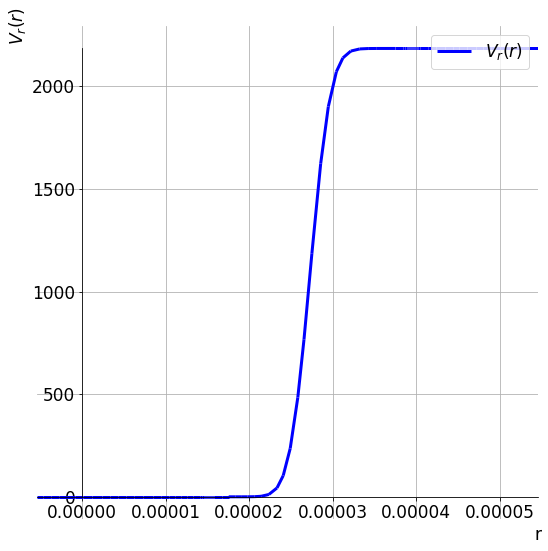
\includegraphics[width=.4\textwidth]{dhd_convergence/analytic_V.png}
\caption{Слева: функция $S(r, t)$ в моменты времени $0$  и $T$ . Справа: функция $V_r(r)$}
\label{fig:dhd_convergence_analytic}
\end{figure}
Задача решается с граничными условиями симметрии слева и камня справа. Аналитические функции решения удовлетворяют условиям симметрии \eqref{eq:symmetry}. Для аппроксимации производной по времени используется метод второго порядка по трем точкам, приведенный в разделе \ref{methods:time_integration}. Поэтому $\tau$ делится пропорционально $h$. Минимальное количество точек D сетки - 20. Задача данного эксперимента - убедиться в асимптотических свойствах сходимости схемы. Поэтому шаг по времени берется достаточно мелким.
\paragraph{Вид источника}
Правые части в уравнении \eqref{eq:dhd_difference} имеют сложный вид и вычисляются с помощью символьной математики. Мы не приводим их здесь, поскольку они заняли бы несколько листов. Приведем графики источников массы и изменения импульса на рис. \ref{fig:dhd_convergence_source}.
\begin{figure}[H]
\centering
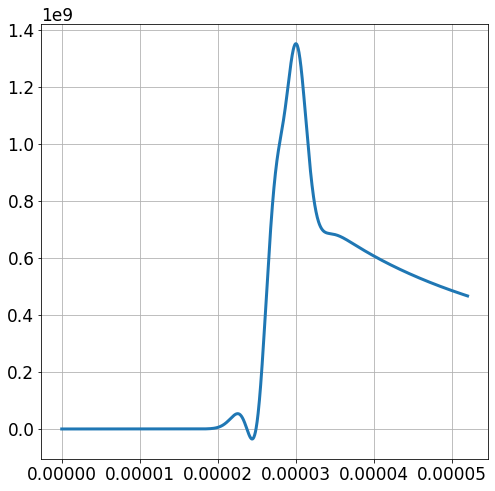
\includegraphics[width=.4\textwidth]{dhd_convergence/source_n.png}
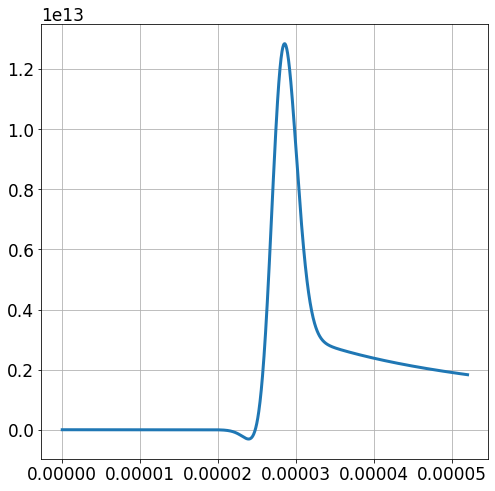
\includegraphics[width=.4\textwidth]{dhd_convergence/source_v.png}
\caption{Источники массы (слева) и изменения импульса (справа) в момент времени $t=T$.}
\label{fig:dhd_convergence_source}
\end{figure}
\paragraph{Результаты}
Результаты исследования приведены на рисунках \ref{fig:dhd_convergence_n0}, \ref{fig:dhd_convergence_n1}, \ref{fig:dhd_convergence_v} для переменных $n_0$, $n_1$ и $V_r$. Рисунки имеют одинаковую структуру. Слева изображен график нормы ошибки в зависимости от шага $h$, справа - зависимость нормы ошибки от времени. Везде используется норма $L_2$ по всему пространству в один момент времени.
\begin{figure}[H]
\centering
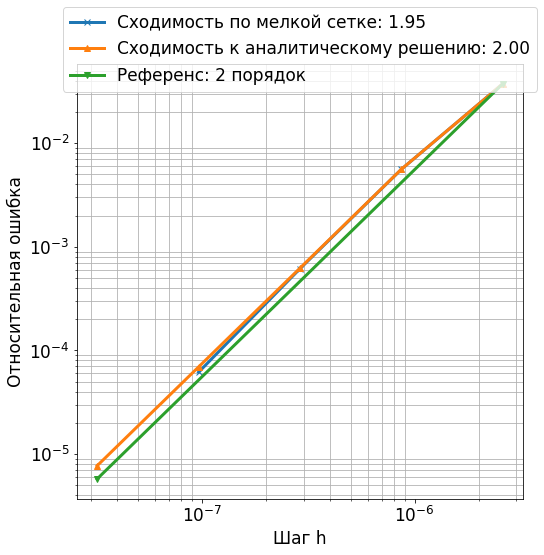
\includegraphics[width=.5\textwidth]{dhd_convergence/convergence_n0.png}\hfill
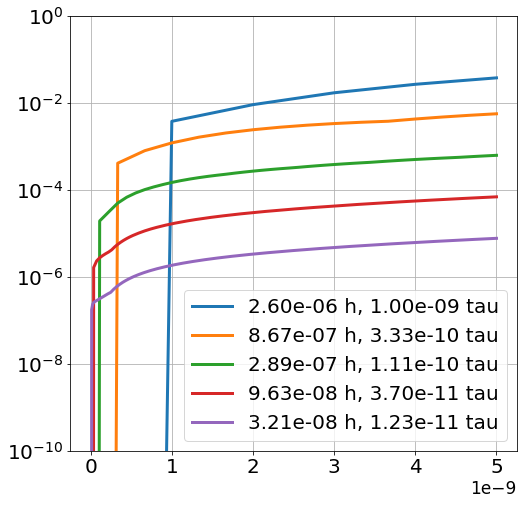
\includegraphics[width=.5\textwidth]{dhd_convergence/time_error_n0.png}
\caption{Слева: зависимость нормы ошибки от сетки при $t = T$ для $n_0$. Справа: зависимость ошибки от времени для $n_0$.}
\label{fig:dhd_convergence_n0}
\end{figure}

\begin{figure}[H]
\centering
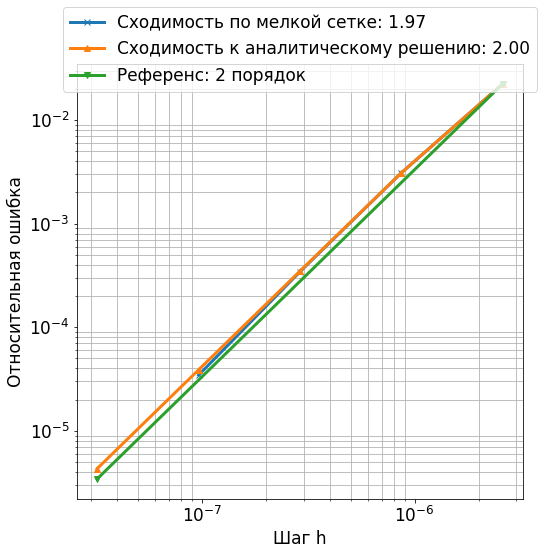
\includegraphics[width=.5\textwidth]{dhd_convergence/convergence_n1.png}\hfill
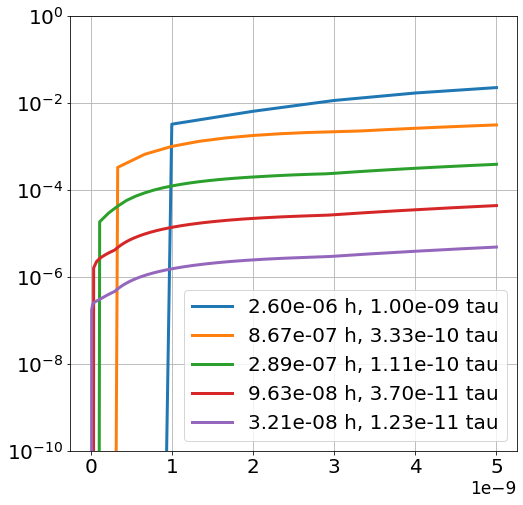
\includegraphics[width=.5\textwidth]{dhd_convergence/time_error_n1.png}
\caption{Слева: зависимость нормы ошибки от сетки при $t = T$ для $n_1$. Справа: зависимость ошибки от времени для $n_1$.}
\label{fig:dhd_convergence_n1}
\end{figure}

\begin{figure}[H]
\centering
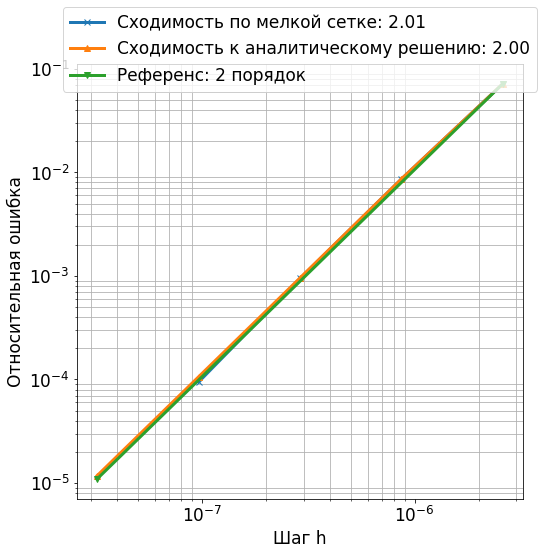
\includegraphics[width=.5\textwidth]{dhd_convergence/convergence_v.png}\hfill
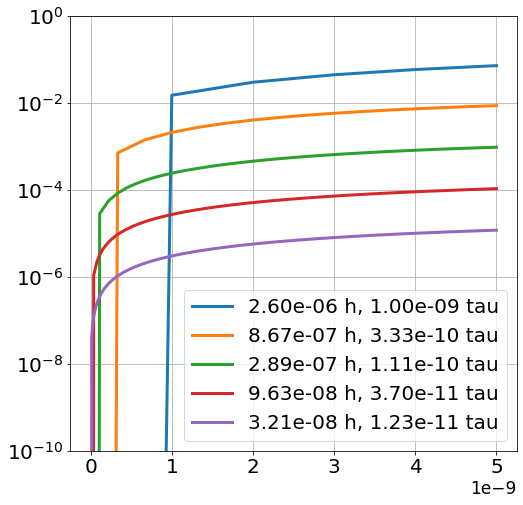
\includegraphics[width=.5\textwidth]{dhd_convergence/time_error_v.png}
\caption{Слева: зависимость нормы ошибки от сетки при $t = T$ для $V_r$. Справа: зависимость ошибки от времени для $V_r$.}
\label{fig:dhd_convergence_v}
\end{figure}

На рис. \ref{fig:dhd_convergence_error} приведена ошибка в последний момент времени для самой точной сетки. Значения нормированы на мольную плотность в чистой фазе.
\begin{figure}[H]
\centering
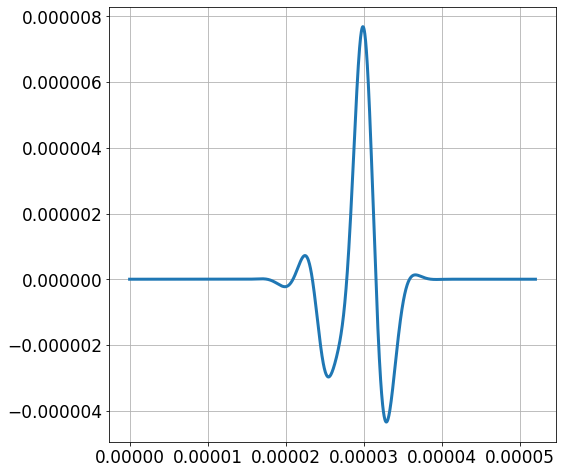
\includegraphics[width=.5\textwidth]{dhd_convergence/rel_err_n0.png}\hfill
\caption{Слева: зависимость нормы ошибки от сетки при $t = T$ для $n_0$. Справа: зависимость ошибки от времени для $n_0$.}
\label{fig:dhd_convergence_error}
\end{figure}
\subsubsection{Сравнение шага по времени неявной схемы при разных скоростях \label{dhd:t_tau}}
Для явной схемы шаг по времени ограничен условием устойчивости независимо от скорости процессов в системе. Для неявной схемы нет такого ограничения, однако при слишком большом шаге $\tau$ метод Ньютона может не сойтись. Поэтому шаг по времени все еще ограничен, хоть и на несколько порядков слабее. Это ограничение зависит от скорости процессов преобладающих в системе.
\par
Цель данного эксперимента - измерить, с каким максимальным шагом $\tau$ может идти расчет по неявной схеме. Моделируются течения с разными скоростями в области со сферической симметрией.

\subsubsection*{Постановка эксперимента} 
Капля первой жидкости расположена в центре. Ее окружает вторая жидкость. На внешней границе области расположен источник, который закачивает вторую жидкость с постоянной интенсивностью. В центре находится труба, которая поддерживает постоянную концентрацию первой жидкости, убирая излишек. Вторая жидкость вытесняет первую, и граница между двумя жидкостями постепенно приближается к центру симметрии.
\begin{figure}[H]
\centering
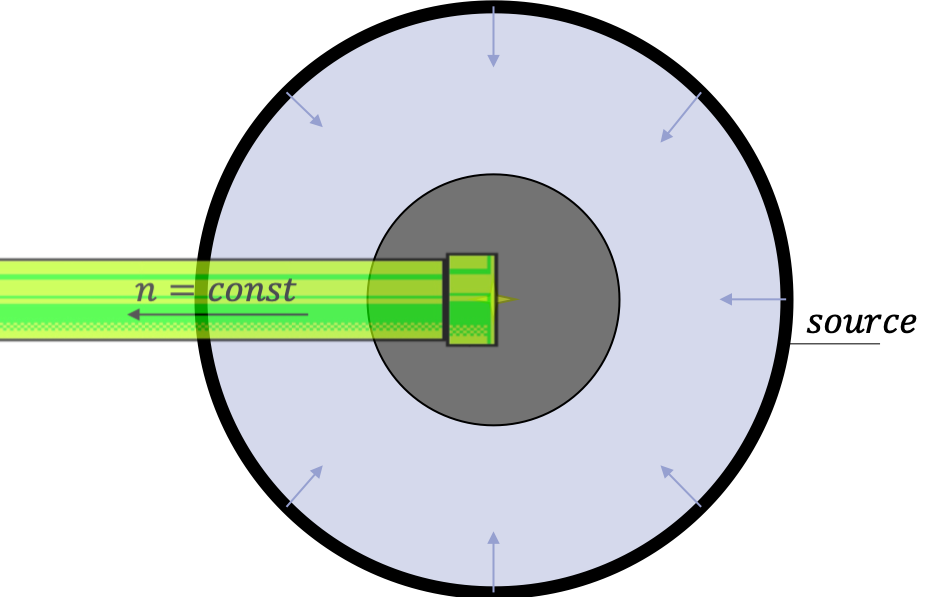
\includegraphics[width=0.5\textwidth]{dhd_t_tau/tube_experiment.png}
\caption{Постановка эксперимента.}
\end{figure}
С точки зрения численной схемы, постановка выглядит так:
\begin{itemize}
\item Граничные условия: \textit{Дирихле} слева и \textit{камень} справа
\item Начальное условие --- стационарное распределение из эксперимента \ref{dhd:interface}
\item Точечный источник массы на правой границе с постоянной интенсивностью, меняющейся от эксперимента к эксперименту
\end{itemize}

\subsubsection*{Результаты}
На рис. \ref{fig:t_tau} снизу приведена зависимость максимальной скорости в задаче от времени симуляции. Это скорость движения границы между жидкостями. Скорость пропорциональна интенсивности источника. На верхнем графике \ref{fig:t_tau} зависимость $\tau$ от времени симуляции. Шаг $\tau$ измеряется в секундах.
Расчет начинается с маленького шага, который плавно повышается, если методу Ньютона удалось сойтись. Так мы выходим на планку, показывающую максимальный шаг при данной скорости процесса. Для смеси жидкостей с используемыми параметрами шаг явной схемы, при котором симуляция остается устойчивой, $\tau_{\textrm{explicit}} \sim 10^{-9}$ с.
\begin{figure}[H]
\centering
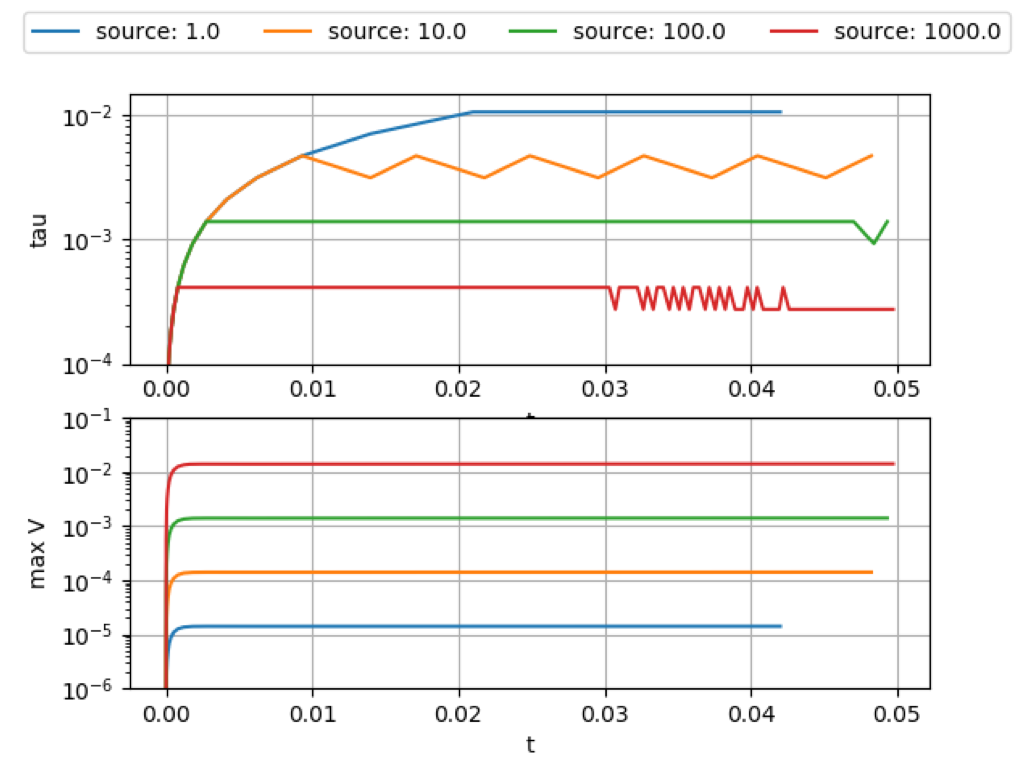
\includegraphics[width=0.8\textwidth]{dhd_t_tau/t_tau.png}
\caption{Зависимость $\tau$ от времени симуляции при различных скоростях}
\label{fig:t_tau}
\end{figure}
Полученный результат подтверждает гипотезу о зависимости шага симуляции по времени $\tau$ от скорости процессов в системе. Это значит, что использование неявной схемы будет наиболее эффективно в течениях двух жидкостей, где преобладает процесс переноса массы.
\par
Даже с достаточно большой среднемассовой скоростью шаг по времени на 5 порядков превосходит шаг для явной схемы. Нужно отметить, что при сильной диффузии ограничение шага по времени будет существеннее.  Во многих практических задачах большую часть симуляции перенос массы преобладает над диффузионными процессами. Именно в эти моменты неявная схема будет максимально эффективна.
